\documentclass[conference]{IEEEtran}
\usepackage{cite}
\usepackage{amsmath,amssymb,amsfonts}
\usepackage{algorithmic}
\usepackage{graphicx}
\usepackage{textcomp}
\usepackage{xcolor}
\usepackage{booktabs}
\usepackage{float}


\def\BibTeX{{\rm B\kern-.05em{\sc i\kern-.022em b}\kern-.08em
    T\kern-.1667em\lower.7ex\hbox{E}\kern-.125emX}}

\begin{document}

\title{Visualization Tool for Energy Analysts using CIA Dataset}
\author{
    Harshavardhan Dharman\\
    \scriptsize Eindhoven University of Technology\\
    \scriptsize h.dharman@student.tue.nl
\and
    Surya Kannan\\
    \scriptsize Eindhoven University of Technology\\
    \scriptsize s.kannan@student.tue.nl
\and
    Shashank Venkatesha\\
    \scriptsize Eindhoven University of Technology\\
    \scriptsize s.venkatesha@student.tue.nl
\and
    Leela Karthikeyan Haribabu\\
    \scriptsize Eindhoven University of Technology\\
    \scriptsize l.k.haribabu@student.tue.nl
}



\maketitle
\textcolor{blue}{
\begin{abstract}
The Energy Analytics Visualization Tool is a simple intelligence platform specifically designed to provide energy analysts with a unified environment for cross-sectoral discovery and infrastructure assessment. By integrating five multidisciplinary datasets, the tool enables the analyst to transition seamlessly from geographic overviews to deep multivariate profiling using Coordinated Multiple Views, such as Choropleth Maps, Top-N Rankings, and PCA Cluster plots that reveal hidden peer groups of nations with shared industrial footprints. This design prioritizes "details-on-demand," allowing the user to investigate how physical assets like pipelines and generating capacity drive economic output while highlighting critical structural dependencies essential for policy mapping. Using a comprehensive dataset of over 200 nations, we analyze the critical intersections of carbon intensity, energy security, and universal access. Our findings reveal that global $CO_{2}$ emissions are heavily concentrated in five key nations, yet "carbon intensity" (emissions per unit of GDP) reveals a different set of industrial challenges in developing economies. Furthermore, we identified a moderate correlation (0.46) between national wealth and energy access, highlighting that infrastructure gaps persist despite economic growth.  By exposing these kinds of insight through interactive Parallel Coordinates and heatmaps, the platform empowers the energy analyst to pinpoint "efficiency frontiers" where nations optimize resource allocation. Ultimately, this visualization environment exposes complex industrial inter-dependencies that traditional, static statistical models often obscure, providing the analyst with a dynamic tool for evidence-based decision-making.
\end{abstract}
}

\begin{IEEEkeywords}
Energy Analytics, Information Visualization, Multivariate Profiling, Infrastructure Assessment, PCA Clustering.
\end{IEEEkeywords}

\section{Introduction}
\subsection{Motivation and Domain Problem}
In an era of unparalleled global interconnection, there is a challenge in understanding the complex relationships between energy production, economic development, infrastructure, and environmental sustainability across all countries. Traditional statistical tables and reports fail to reveal the nuanced patterns, regional clusters, and multi-dimensional correlations that drive the interdependent link between energy usage and economic growth. The primary domain goal for the energy analyst is to understand how physical energy infrastructure, such as generating capacity and pipelines, correlates with economic health, and to identify patterns such as "high GDP but high carbon intensity" or "expanding infrastructure combined with low energy equity." Current approaches like spreadsheets and static reports make it hard to see these patterns; interactive visualization is well-suited because it leverages spatial position, color, and length as highly effective perceptual channels for comparison and pattern finding.

\subsection{Target Users and Goals}
\textbf{Target User:} The primary user of this tool is the Energy Analyst tasked with synthesizing complex, multi-sector data to guide infrastructure planning and policy decisions.

\textbf{Project Goals:} The primary goal is to facilitate exploration and analysis by allowing the analyst to investigate how energy mixes and transport networks support population growth while driving national economic health. Through interactive features like PCA clustering, the tool enables the user to identify "peer nations" with similar industrial footprints. Ultimately, the Visualization Tool allows the analyst to pinpoint "connectivity gaps" and discover "positive deviants" who successfully decouple economic growth from high environmental impact.

\subsection{Why Visualization?}
Visualization serves as a critical cognitive bridge between raw, high-dimensional data and strategic decision-making by transforming abstract numbers into actionable relational patterns. While traditional statistical summaries often operate as black boxes'' that hide nuanced outliers, a visual interface enables Human-in-the-loop'' discovery, allowing an analyst to navigate the complex interdependencies of infrastructure, economics, and environmental impact. By offloading cognitive load to the human visual system optimized for pattern recognition and the analyst can solve high-stakes problems invisible in tabular formats, such as identifying efficiency frontiers where nations decouple growth from carbon intensity, assessing supply chain vulnerabilities, and uncovering infrastructure equity gaps where rising wealth fails to translate into universal energy access. Ultimately, visualization empowers the analyst to move beyond observing data to generating and testing hypotheses for evidence-based policy mapping that static algorithmic outputs cannot achieve.

\section{Data Analysis}

\subsection{Domain Data Specification}
The visualization utilizes the CIA World Factbook, a comprehensive dataset containing statistical profiles for over 200 countries at the intersection of infrastructure and macroeconomics. Nations are analyzed through five key dimensions:

\textbf{Energy:} Quantifies resource footprints through electricity access, generating capacity, and fossil fuel metrics (coal, gas, petroleum). $CO_2$ emissions are included to evaluate industrial sustainability.


\textbf{Economy:} Measures financial health and industrial scale using absolute values like Real GDP (PPP) and Trade Volume (Exports/Imports), alongside GDP per Capita for relative prosperity.


\textbf{Demographics:} Uses Total Population as the primary metric to contextualize energy demand and the scale of required infrastructure.


\textbf{Transportation:} Focuses on physical connectivity via gas and oil pipeline mileage (km), reflecting the technological maturity of a nation’s distribution networks.


\textbf{Geography:} Defines the physical context through Total/Land Area and land-use types like Forest and Agricultural Land to assess resource potential and spatial constraints.

In our approach, we have synthesized a multi-domain dataset by merging five distinct categories of country-level indicators: Energy, Economy, Demographics, Transportation, and Geography. Each observation in the final processed dataset represents a sovereign state, identified by its unique ISO-Alpha 3 code. To ensure global coverage and facilitate spatial visualization, we performed a name-matching operation between the CIA World Factbook records and the Gapminder ISO database, resolving nomenclature discrepancies (e.g., mapping "Czechia" to the "Czech Republic" to maintain consistency across historical and modern records).

\subsection{Data Abstraction}
All The datasets are abstracted according to Munzner's data model framework, as shown in following tables.

\begin{table}[h]
\centering
\caption{Energy Dataset Abstraction}
\label{tab:data_abstraction}
\small
\begin{tabular}{|p{3.7cm}|p{1.5cm}|p{0.9cm}|p{1.4cm}|}
\hline
\textbf{Attribute} & \textbf{Semantic Type} & \textbf{Data Type} & \textbf{Range} \\
\hline
Country & Categorical & Key (Item) & 260 unique \\
electricity\_access\_percent & Quantitative & Ratio & 0--100\% \\
elec\_generating\_capacity\_kW & Quantitative & Ratio & 0--2.38B \\
coal\_metric\_tons & Quantitative & Ratio & 0--3.69B \\
petroleum\_bbl\_per\_day & Quantitative & Ratio & 0--18.6M \\
refined\_petrol\_products & Quantitative & Ratio & 0--20.3M \\
refined\_petrol\_exports & Quantitative & Ratio & 0--5.92M \\
refined\_petrol\_imports & Quantitative & Ratio & 0--2.19M \\
natural\_gas\_cubic\_m & Quantitative & Ratio & 0--967B \\
carbon\_dioxide\_emissions & Quantitative & Ratio & 0--11.5B Mt \\
iso\_alpha (derived) & Categorical & Key & 200+ unique \\
continent (derived) & Categorical & Ordered & 6 categories \\
\hline
\end{tabular}
\end{table}

\begin{table}[htbp]
\centering
\caption{Economy Dataset Abstraction}
\small
\begin{tabular}{|l|l|l|l|}
\hline
\textbf{Attribute} & \textbf{Semantic Type} & \textbf{Data Type} & \textbf{Range} \\
\hline
Real GDP (PPP) & Quantitative & Ratio & 0--23,320 \\
GDP per Capita & Quantitative & Ratio & 0--115,700 \\
Exports (B USD) & Quantitative & Ratio & 0--3,527 \\
Imports (B USD) & Quantitative & Ratio & 0--3,401 \\
\hline
\end{tabular}
\end{table}

\begin{table}[htbp]
\centering
\caption{Demographics Dataset Abstraction}
\small
\begin{tabular}{|l|l|l|l|}
\hline
\textbf{Attribute} & \textbf{Semantic Type} & \textbf{Data Type} & \textbf{Range} \\
\hline
Total Population & Quantitative & Absolute & 0--1.42B \\
\hline
\end{tabular}
\end{table}

\begin{table}[htbp]
\centering
\caption{Energy Production Summary}
\small
\begin{tabular}{|l|l|l|l}
\hline
Source & Type & Global Share \\
\hline
Coal & Fossil & High \\
Oil & Fossil & Medium \\
Renewables & Clean & Growing \\
\hline
\end{tabular}
\end{table}

\begin{table}[htbp]
\centering
\caption{Task Abstraction Mapping}
\small
\begin{tabular}{|l|l|l|l}
\hline
Task & Action & Visualization \\
\hline
Emission Analysis & Discover & Choropleth Map \\
Market Control & Compare & Bar Chart \\
Pattern Detection & Analyze & Scatter Plot \\
\hline
\end{tabular}
\end{table}

\section{Task Analysis}
\subsection{Domain-Specific Tasks}
\textbf{Task 1: Analyze Environmental Impact and Global Emissions}
\begin{itemize}
    \item \textbf{Description}: Identifying drivers of greenhouse gas emissions by analyzing $CO_{2}$ output in relation to industrial scale (see Fig.~\ref{fig:global_emissions}).
    \item \textbf{Why it matters}: Monitoring carbon footprints is essential for assessing global climate policy and identifying heavy polluters.
    \item \textbf{Questions}: Who are the leading global carbon emitters? Which countries contribute most to global $CO_{2}$ emissions? Is there a correlation between electricity capacity and carbon output?
\end{itemize}

% Using [H] to lock the figure precisely after the list
\begin{figure}[H]
    \centering
    % Note: It is best practice to avoid spaces in filenames, e.g., fig_2.jpeg
    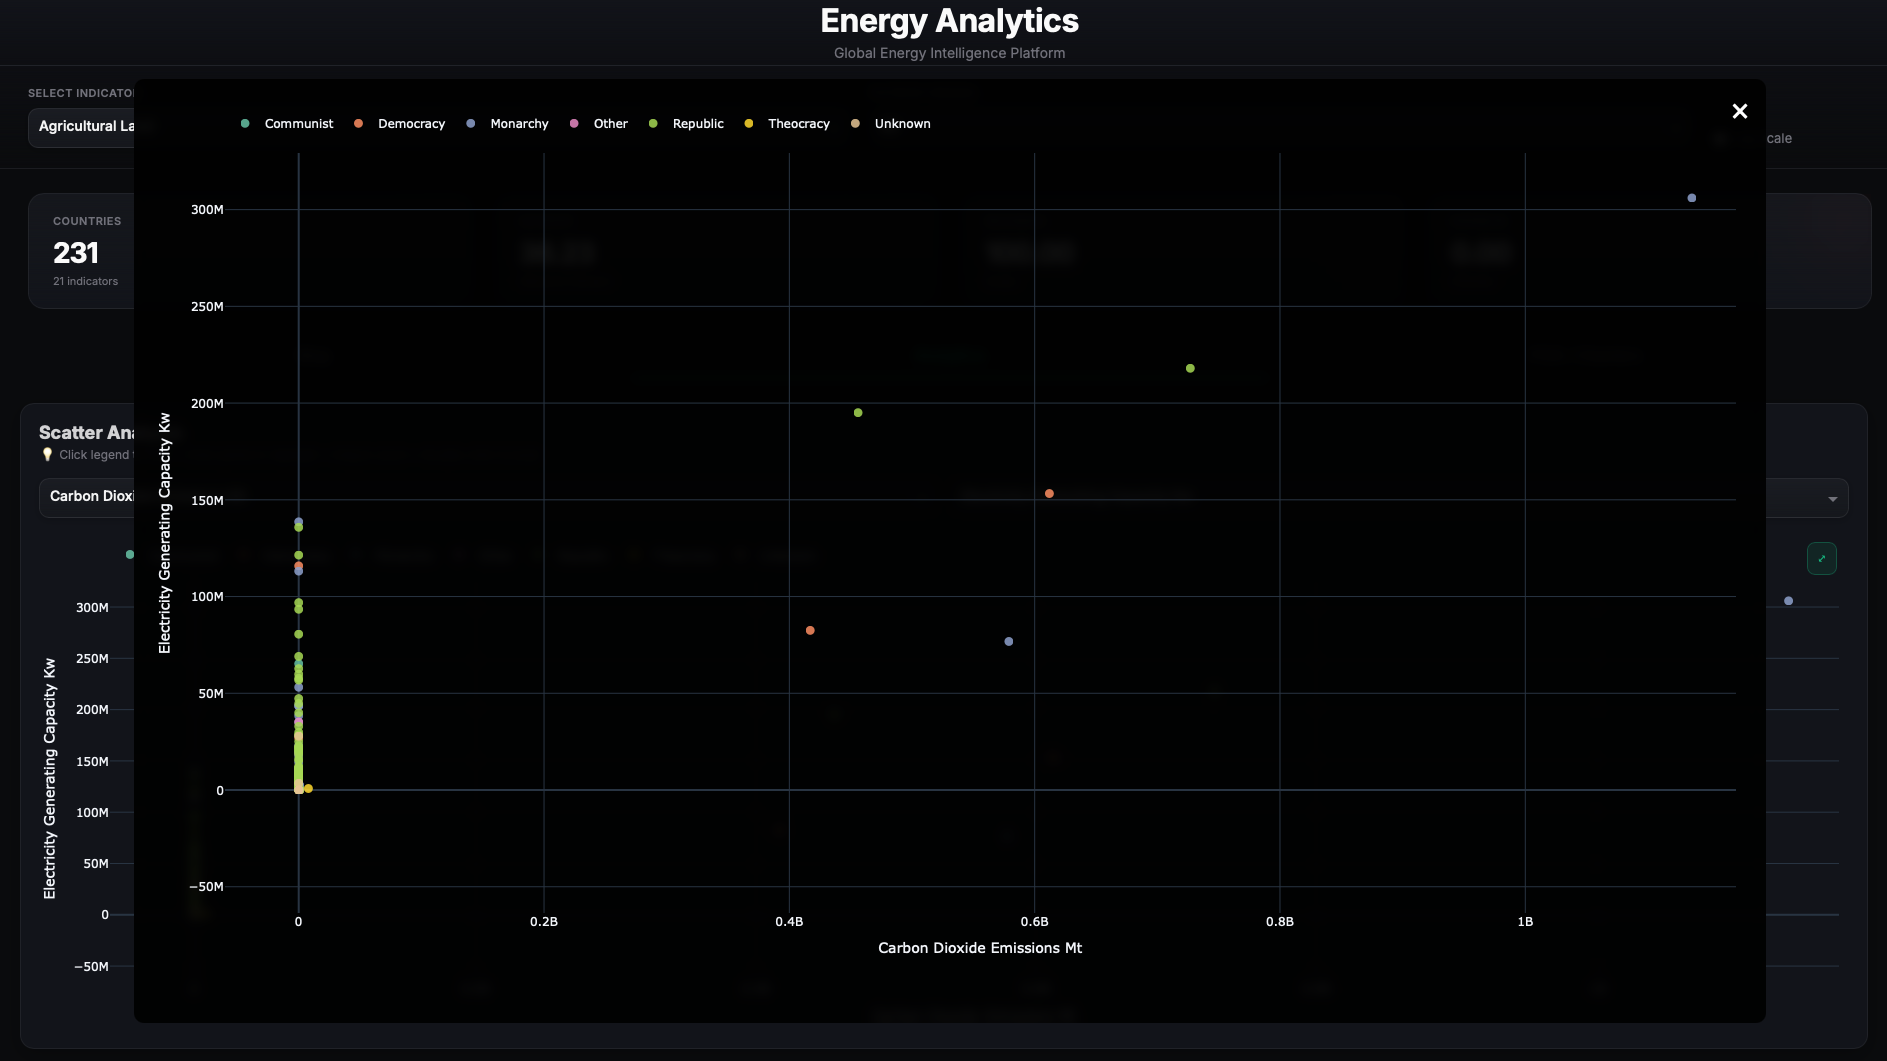
\includegraphics[width=1.0\linewidth]{fig2new.jpeg}
    \caption{Global $CO_{2}$ Emissions vs. Industrial Capacity by Nation.}
    \label{fig:global_emissions}
\end{figure}

\textbf{Task 2: Correlate Economic Wealth and Energy Access}
\begin{itemize}
    \item \textbf{Description}: Investigating if wealth alone is a sufficient driver for infrastructure (see Fig.~\ref{fig:wealth_access}).
    \item \textbf{Questions}: Does economic wealth guarantee energy access? Is there a strong correlation between $GDP$ per capita and electricity access?
    \item \textbf{Insight}: Moderate correlation (0.46). Higher GDP helps, but policy and geography are equally critical.
\end{itemize}

% [H] tells LaTeX: "Put this EXACTLY HERE, do not let it float"
\begin{figure}[H]
    \centering
    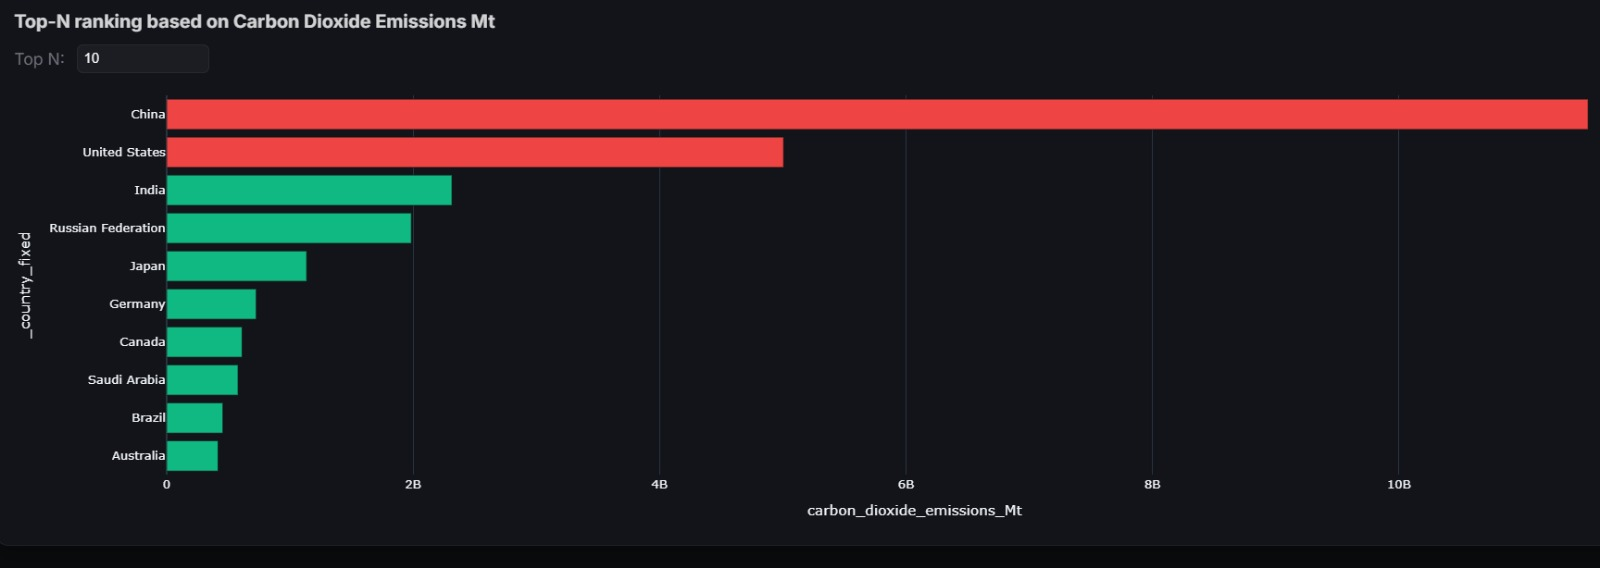
\includegraphics[height = 100, width=1.0\linewidth]{fig3.jpeg}
    \caption{Correlation between GDP per Capita and National Electricity Access.}
    \label{fig:wealth_access}
\end{figure}

\textbf{Task 3: Analyze Carbon Intensity and Economic Efficiency}
\begin{itemize}
    \item \textbf{Description}: Evaluating efficiency by calculating $CO_{2}$ emissions relative to GDP (see Fig.~\ref{fig:carbon_intensity}).
    \item \textbf{Questions}: Which economies are the most "Carbon Intensive"? Who emits the most relative to economic output?
    \item \textbf{Insight}: China and Russia lead major economies. Small island nations show high ratios due to fossil fuel import reliance.
\end{itemize}

% [H] ensures the figure stays directly under the Task 3 bullet points
\begin{figure}[H]
    \centering
    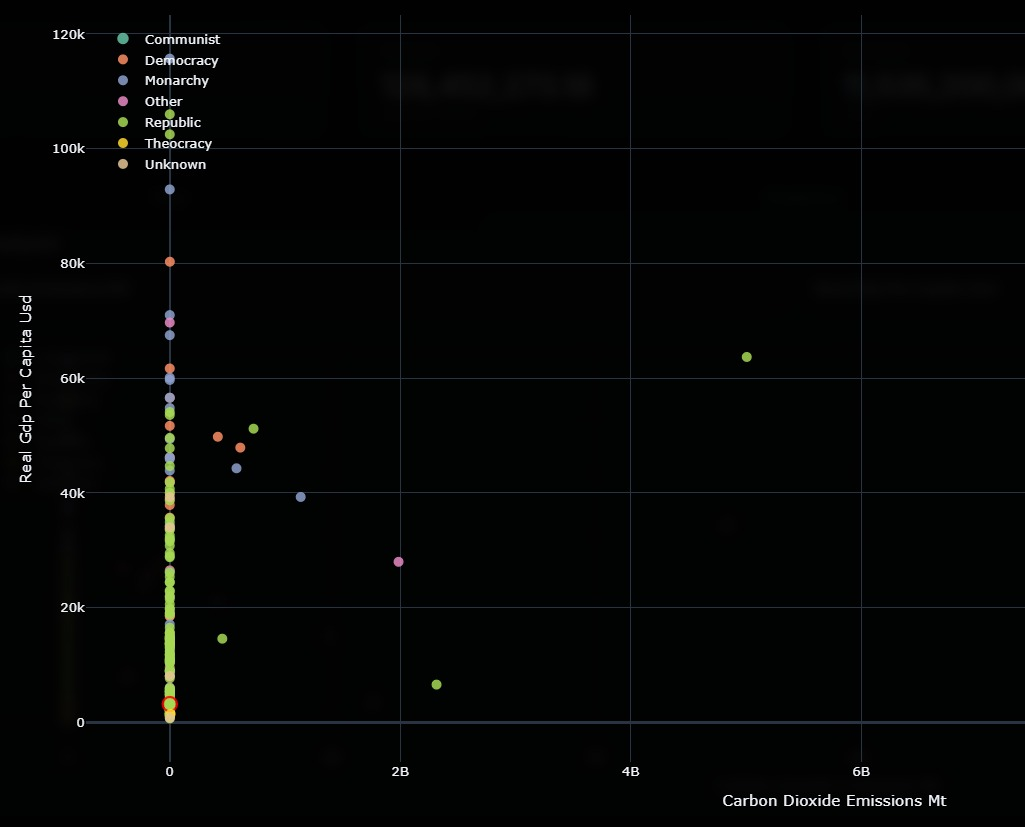
\includegraphics[width=1.0\linewidth]{fig5.jpeg}
    \caption{Real GDP vs Carbon Dioxide Emission Mt.}
    \label{fig:carbon_intensity}
\end{figure}

\subsection{Task Abstraction}
 Following Munzner’s "Why" framework, we abstract the domain-specific tasks into generic action-target pairs. This process removes domain-specific language by shifting from "Energy" or "GDP" to "Distributions," "Dependencies," and "Correlations" by ensuring that the chosen visual encodings are mathematically and perceptually sound. By mapping these high-level goals to specific actions, we can justify the use of coordinated multiple views (CMV) to handle the multivariate nature of the dataset.

 Example: Identify Extremes (Action: Identify | Target: Extremes): First, the analyst uses the Top-N Bar Chart to identify nations where the ratio of $CO_2$ to $GDP$ is highest(see Fig1). This identifies specific items (e.g., China or the Faroe Islands) that deviate from the global norm.
 
 Locate and Discover Distribution (Action: Locate | Target: Spatial Distribution): The analyst uses the Choropleth map to identify the countries with maximum "Petroleum Imports Per day" (see Fig4). The analyst can specifically use the map to discover Import Deficits. For example, by looking at nations with high GDP but low petroleum production (shaded in lighter colors), the analyst identifies regions that are heavily dependent on foreign energy.


 Explore Dependencies (Action: Analyze | Target: Correlation): Finally, the analyst uses the Scatter Plot to "brush" these high-intensity nations and observe the dependency between the total GDP and Carbon Dioxide Emissions(see Fig3). This reveals whether high intensity is a byproduct of rapid industrialization or a result of inefficient, aging infrastructure.

\begin{table}[h]
\centering
\caption{Task Abstraction: Mapping Domain Tasks to Abstract Actions}
\label{tab:task_abstraction}
\small
\begin{tabular}{|p{1.8cm}|p{1.8cm}|p{1.5cm}|p{2.0cm}|}
\hline
\textbf{Domain Task} & \textbf{Action} & \textbf{Target} & \textbf{Idiom Support} \\
\hline
Discover spatial patterns & Discover & Distribution & Choropleth Map \\
\hline
Generate hypotheses & Discover & Dependency & Scatter Plot \\
\hline
Characterize profiles & Derive & Clusters & PCA + K-Means \\
\hline
Correlate attributes & Identify & Correlation & Scatter Plot, Corr. Matrix \\
\hline
Identify extremes & Identify & Extremes & Bar Chart (Top-N) \\
\hline
Filter by region & Filter & Items & Continent Dropdown \\
\hline
Lookup value & Lookup & Value & Hover Tooltip \\
\hline
Locate country & Locate & Position & Geographic Map \\
\hline
Select \& highlight & Select & Item & Click interaction \\
\hline
Brush range & Filter & Range & Parallel Coordinates \\
\hline
\end{tabular}
\end{table}

\begin{table}[h]
\centering
\caption{Idiom Justification and Theoretical Mapping}
\label{tab:idiom_justification}
\small
\begin{tabular}{|p{2.2cm}|p{5.5cm}|}
\hline
\textbf{Idiom} & \textbf{Justification (Why we use it)} \\
\hline
Choropleth Map & Encodes data into spatial regions via color to reveal geographic distributions. \\
\hline
Scatter Plot & Best for identifying dependencies/trends using high-precision position channels. \\
\hline
PCA + K-Means & Derives and visualizes hidden clusters within multi-dimensional datasets. \\
\hline
Bar Chart & Uses the length channel for accurate magnitude comparison and ranking. \\
\hline
Corr. Matrix & Provides a high-level summary of all statistical relationships via color saturation. \\
\hline
Parallel Coords & Enables multivariate profiling and range-based filtering via interactive brushing. \\
\hline
\end{tabular}
\end{table}



\begin{figure*}[t] % The * makes it span both columns (large image)
    \centering
    % width=0.9\textwidth makes it wide, height=7cm sets the vertical scale
    % keepaspectratio prevents the image from looking stretched
    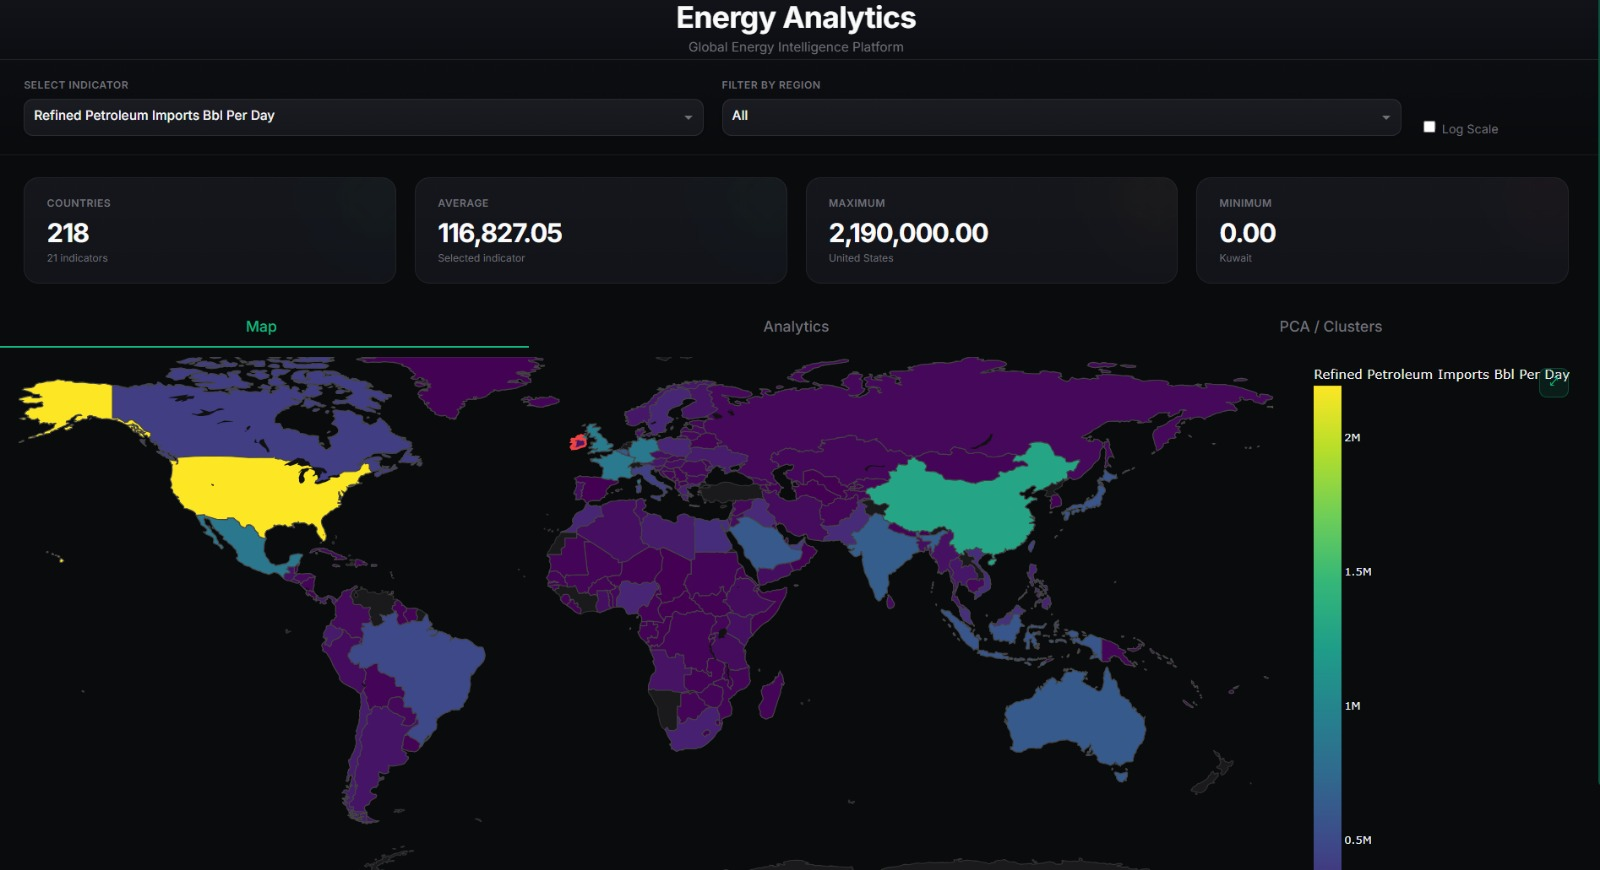
\includegraphics[width=500\textwidth, height=10cm, keepaspectratio]{fig9.jpeg} 
        \caption{Agricultural land view through Choropleth Map}
    \label{fig:multivariate_distribution}
\end{figure*}

\newpage
\section{Visualization Design}


\subsection{Visual Channel Selection}
Our visual encodings follow Munzner's effectiveness rankings for quantitative data. Position is the most effective channel and is used in scatter plots for X and Y axes, in the PCA embedding, and in the choropleth map for spatial location. Length is used in bar charts for ranking comparison. Color saturation and hue are used in the choropleth with a Blues scale for sequential data, in the correlation matrix with a diverging RdBu scale, and for continent-based coloring across all scatter-based views.

\subsection{Interaction Design}
Linked views support Shneiderman's Visual Information Seeking Mantra of overview first, zoom and filter, then details-on-demand. The choropleth map provides an overview showing global energy distribution at a glance. Zoom and filter capabilities are provided through the continent dropdown that filters all views and through parallel coordinates brushing that narrows the displayed range. Details-on-demand are available through hover tooltips that reveal exact values and through the comparison table that provides detailed country profiles. View linking is achieved by clicking a country on the map, which highlights it in scatter plots, PCA, and parallel coordinates bidirectionally.

\section{Use Case: Energy Analyst Exploration}

This section demonstrates an extensive data exploration process conducted by an energy analyst using the tool.

\subsection{Scenario}

An energy analyst at a policy research institute seeks to understand the relationship between energy production, carbon emissions, and electricity access across different regions. The goal is to identify countries that could serve as models for sustainable energy development.

\subsection{Exploration Process}

The analyst begins by viewing electricity access percentage on the choropleth map in Step 1, the overview (see Fig 5). Immediately visible patterns emerge as Europe and North America show near-universal access represented in deep purple, while Sub-Saharan Africa shows significant gaps shown in yellow. The analyst clicks on several African countries to highlight them for further investigation.

\begin{figure}[H]
    \centering
    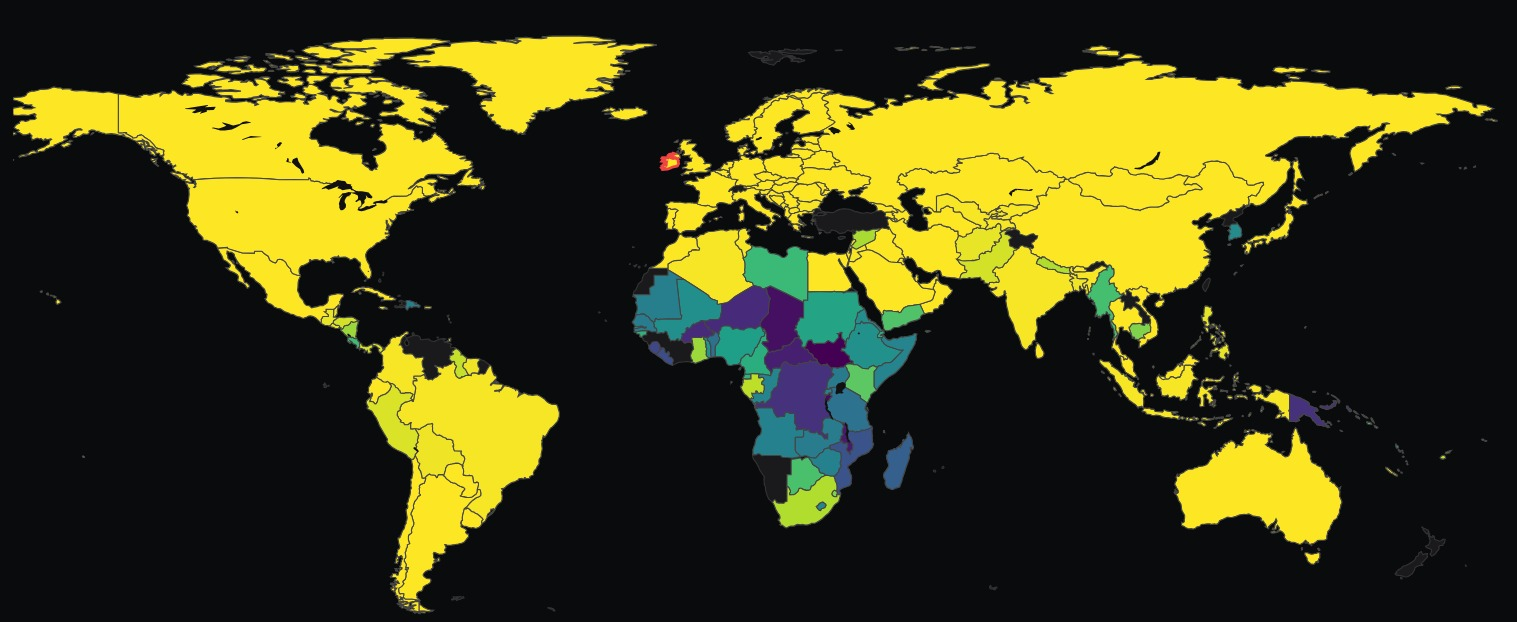
\includegraphics[width=1.0\linewidth]{fig10.jpeg}
    \caption{Electricity Access Percentage}
    \label{fig:placeholder}
\end{figure}


In Step 2, correlation discovery, the analyst switches to the Analytics tab and plots petroleum production in barrels per day on the X-axis against carbon dioxide emissions on the Y-axis (see Fig 6). A strong positive correlation is visible. However, the highlighted African countries from Step 1 appear as outliers with low petroleum production but varying emissions. The analyst identifies Nigeria as an exception showing high petroleum production but relatively moderate emissions.

\begin{figure}[H]
    \centering
    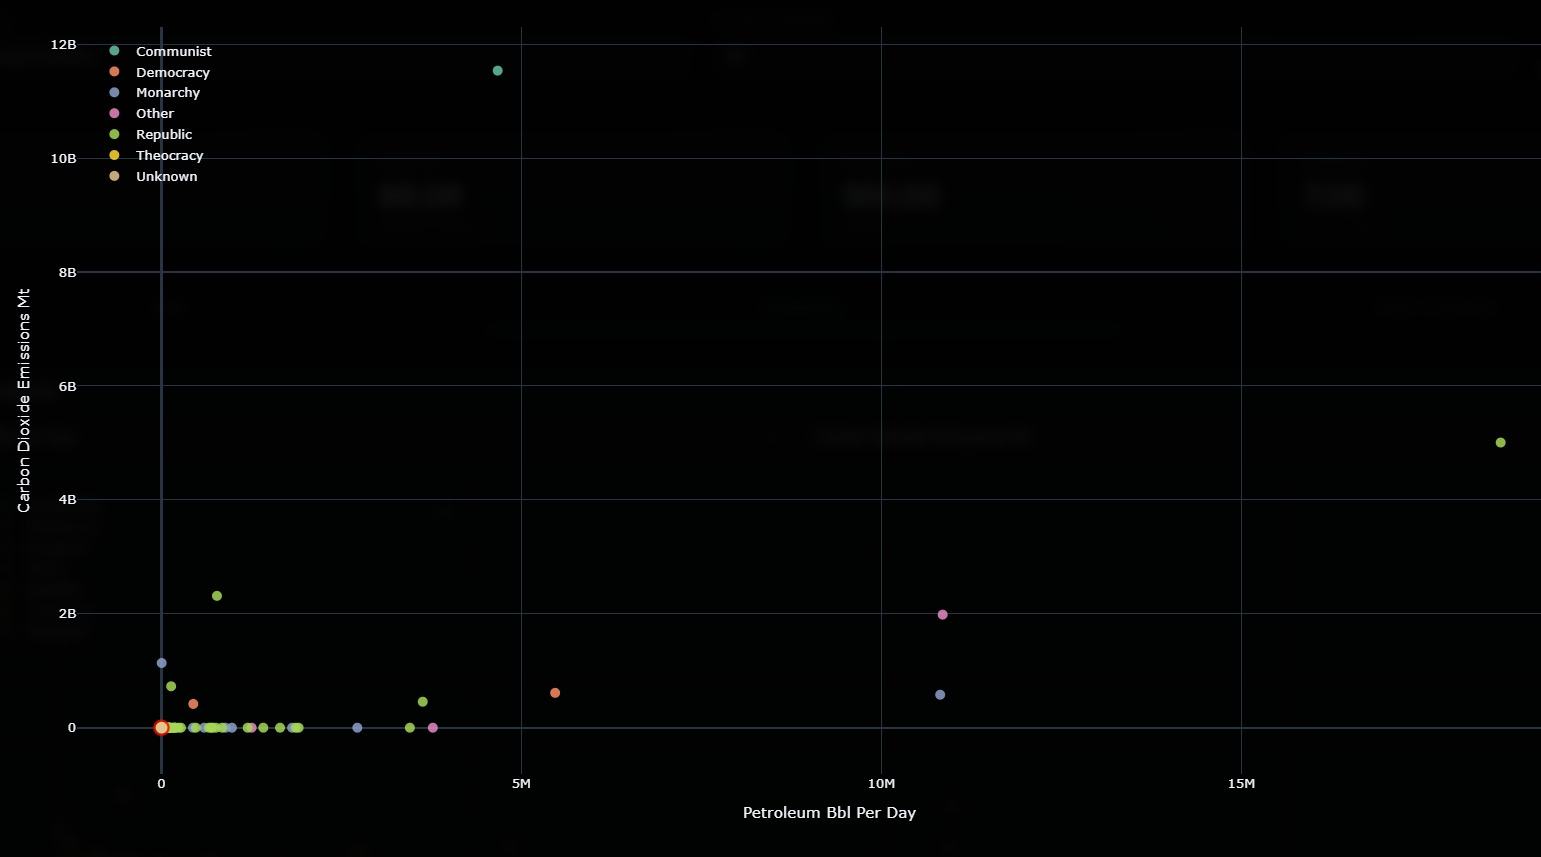
\includegraphics[width=1.0\linewidth]{fig11.jpeg}
    \caption{Petroleum Production vs CO2 Production}
    \label{fig:placeholder}
\end{figure}


Step 3 involves multivariate analysis using parallel coordinates (see Fig 7). Brushing to see highest carbon Dioxide emissions of countries with highest real GDP per capita USD, Australia, Austria and Bahrain were the top among the total countries.

\begin{figure}[H]
    \centering
    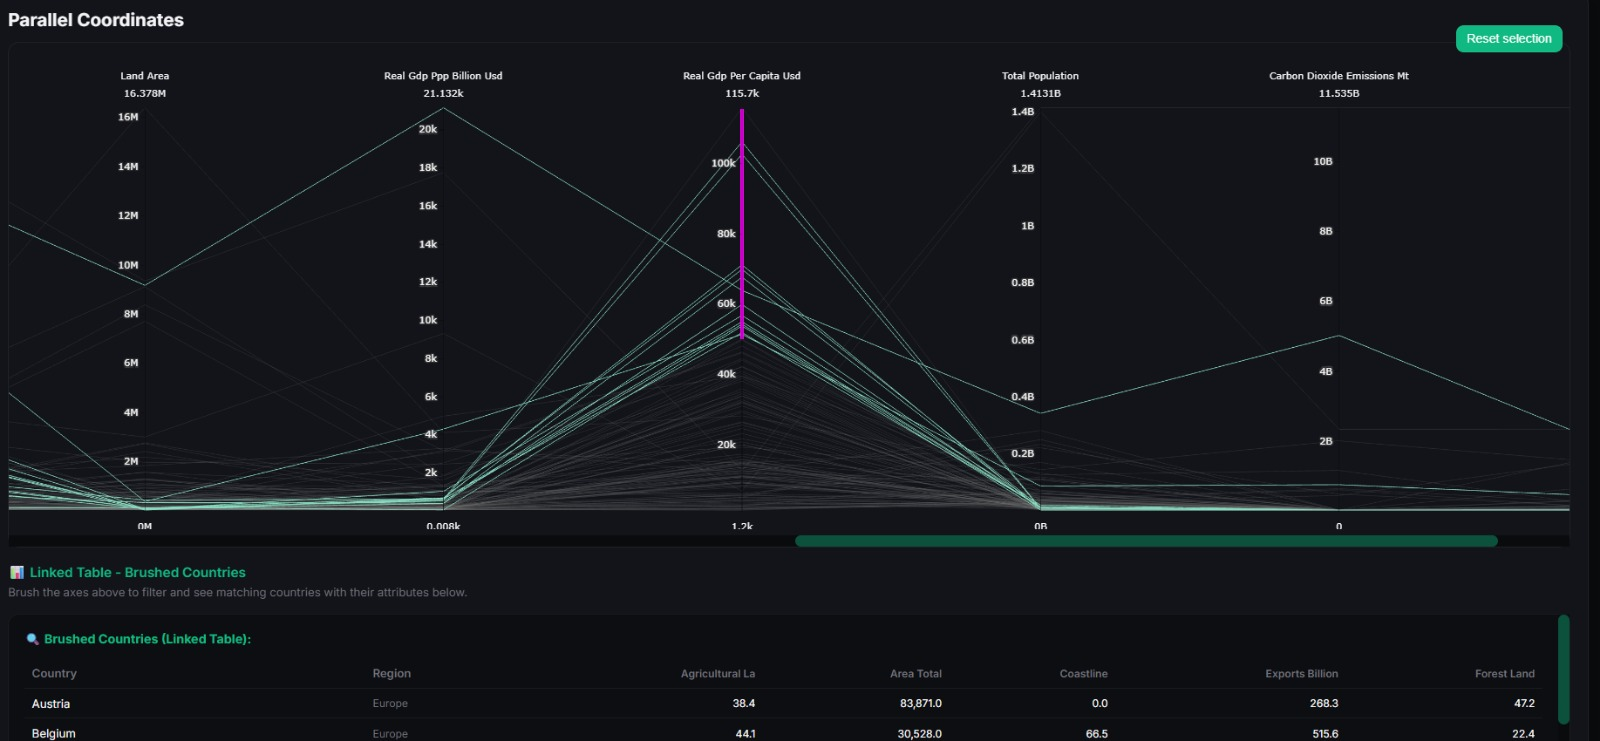
\includegraphics[width=1.0\linewidth, height=5cm, keepaspectratio]{fig12.jpeg}
    \caption{Multivariate Analysis for Real GDP VS Carbon Dioxide emission.}
    \label{fig:pca_clustering}
\end{figure}
Finally, Step 4 involves Correlation Heat Map (See Fig 8), The heatmap shows an exceptionally high positive correlation (typically $>0.90$) between Coal Metric tons and Electricity Generating Capacity ($kW$). This confirms that electricity output is almost perfectly scaled with power infrastructure(coal). For an analyst, this means that "Electricity Demand Forecasting" is directly tied to "Raw Material Demand Forecasting".

\begin{figure}[H]
    \centering
    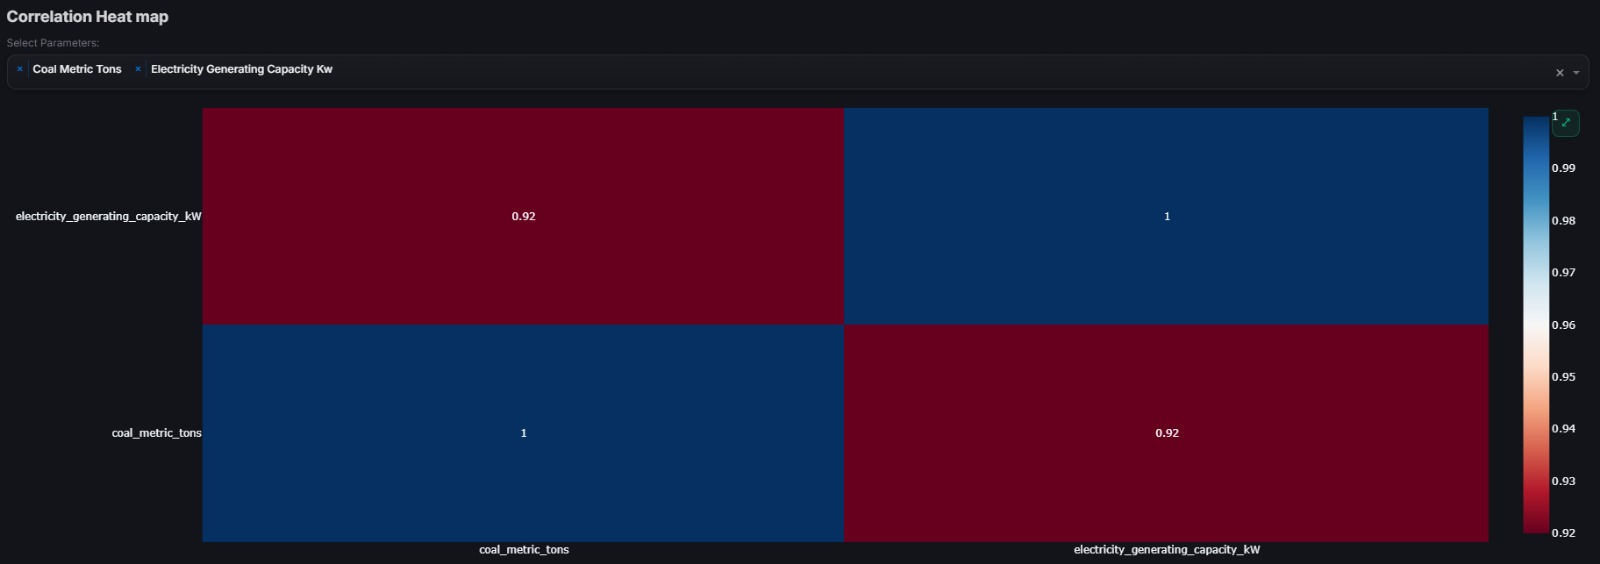
\includegraphics[width=1.0\linewidth]{fig15.jpeg}
    \caption{Electricity Generating Capacity KW through Correlation Heat Map}
    \label{fig:placeholder}
\end{figure}

Analytic Value: It reveals that wealth alone does not guarantee infrastructure parity. This allows the analyst to pinpoint "Efficiency Outliers"—nations that have achieved high energy access despite lower GDP, providing a model for cost-effective infrastructure policy.


Through interactive exploration, the analyst discovered several important findings. First, decoupling energy development from carbon emissions is possible, as several countries achieve near-universal electricity access with low carbon emissions, suggesting that energy development need not be carbon-intensive. Second, regional patterns emerged showing that geographic clustering of energy access gaps aligns with development status but not always with resource availability. 

This exploration process demonstrates how linked views and interaction enable hypothesis generation, pattern discovery, and evidence-based insight extraction, tasks that would be extremely difficult with static tables or isolated visualizations.

\subsection{Future Work}

Several enhancements would strengthen this visualization tool. A temporal slider incorporating historical data would enable time-series comparison to track how countries' energy profiles evolve. Computing derived attributes such as per-capita and efficiency metrics by merging with demographic data would deepen analytical capabilities. Axis reordering allowing users to drag axes in parallel coordinates for correlation-based ordering would improve the multivariate view. Export functionality enabling analysts to export filtered subsets for external analysis would support integration with other tools. Finally, guided tours providing preset exploration paths for common analytical scenarios would help new users learn the system effectively.

\section{Implementation}
The tool is implemented entirely in Python, using Dash for web-based UI construction and Plotly for interactive visualizations. Data cleaning employs Pandas and regular-expression–based preprocessing. ISO code and continent inference use external libraries such as pycountry, pycountry convert, and gapminder. To achieve Multi View coordination, Dash creates Callbacks that link the state (i.e., clickData, relayoutData, and dcc.Store) of the respective components together. The technical challenges we encountered while developing the system included inconsistent Country names from the CIA database; Missing or Non-numeric; Handling large heterogeneous datasets; Maintaining a uniform display of a stable map (as it would be used from interaction through either brushing methodology); Linking map and scatter selection using ISO-code matching; Designing a Dark-Themed Responsive UI with animated transition, Full-Screen modal, and Vertical Scrollable Containers. The final system integrates all components cohesively while remaining modular for future extension. Screenshots of the implemented visualizations are provided in Appendix

\section{Conclusion and Future Work}

\subsection{Summary of Results}

This project developed an interactive visualization tool that enables energy analysts to explore the CIA Energy Dataset across 260 countries. The tool successfully supports a hierarchy of analytical tasks from high-level pattern discovery to low-level value retrieval through coordinated multiple views including choropleth maps, scatter plots, parallel coordinates, PCA clustering, and comparison tables.

\subsection{Benefits and Limitations}

The tool offers several important benefits. Linked views enable seamless exploration from overview to detail, allowing analysts to quickly drill down into specific countries of interest. Multiple visualization idioms support different task types including comparison, correlation analysis, and clustering. Interactive filtering allows hypothesis testing through selection and brushing operations. The dark theme with animations provides a professional and modern user experience.

However, several limitations should be noted. The CIA dataset represents a single point in time, preventing temporal trend analysis that would reveal how energy profiles have changed over years. Approximately 15 percent of country-indicator pairs contain missing values, reducing coverage for some nations. Additionally, the lack of derived metrics such as emissions per capita or emissions per kilowatt-hour limits the depth of analysis, as these ratios would provide additional insight but require external population and GDP data.

\subsection{Reflection on Design Choices}

Our initial choice of a choropleth map proved effective for revealing spatial patterns in electricity access, as the geographic encoding immediately communicated regional disparities. However, for attributes without clear geographic patterns such as natural gas production, a sorted bar chart would be more effective.

The parallel coordinates view, while powerful for multivariate filtering, suffers from axis overlap when all nine indicators are displayed. Allowing users to reorder or subset axes would improve usability. The PCA clustering successfully revealed country groupings but lacks interpretability, and adding loading vectors would help analysts understand which attributes drive cluster separation.

\textcolor{blue}{
\begin{thebibliography}{00}
\bibitem{munzner2014} T. Munzner, ``Visualization Analysis and Design,'' A K Peters/CRC Press, 2014.
\bibitem{shneiderman1996} B. Shneiderman, ``The eyes have it: a task by data type taxonomy for information visualizations,'' in Proceedings 1996 IEEE Symposium on Visual Languages, pp. 336-343, 1996.
\bibitem{plotly} Plotly Technologies Inc., ``Plotly Python Graphing Library,'' \url{https://plotly.com/python/}, 2024.
\bibitem{dash} Plotly Technologies Inc., ``Dash: A Python Framework for Building Analytical Web Applications,'' \url{https://dash.plotly.com/}, 2024.
\bibitem{cia} Central Intelligence Agency, ``The World Factbook,'' \url{https://www.cia.gov/the-world-factbook/}, 2024.
\bibitem{sklearn} F. Pedregosa et al., ``Scikit-learn: Machine Learning in Python,'' Journal of Machine Learning Research, vol. 12, pp. 2825-2830, 2011. (Used for PCA and K-Means clustering)
\bibitem{pandas} W. McKinney, ``Data Structures for Statistical Computing in Python,'' in Proceedings of the 9th Python in Science Conference, pp. 51-56, 2010.
\bibitem{pycountry} ``pycountry: ISO country, subdivision, language, currency and script definitions,'' \url{https://pypi.org/project/pycountry/}, 2024.
\end{thebibliography}
}
\end{document}